\section{Ocelotl Tool and Trace Visualization}
\vfill
\centering
\begin{minipage}[c]{0.70\textwidth}
  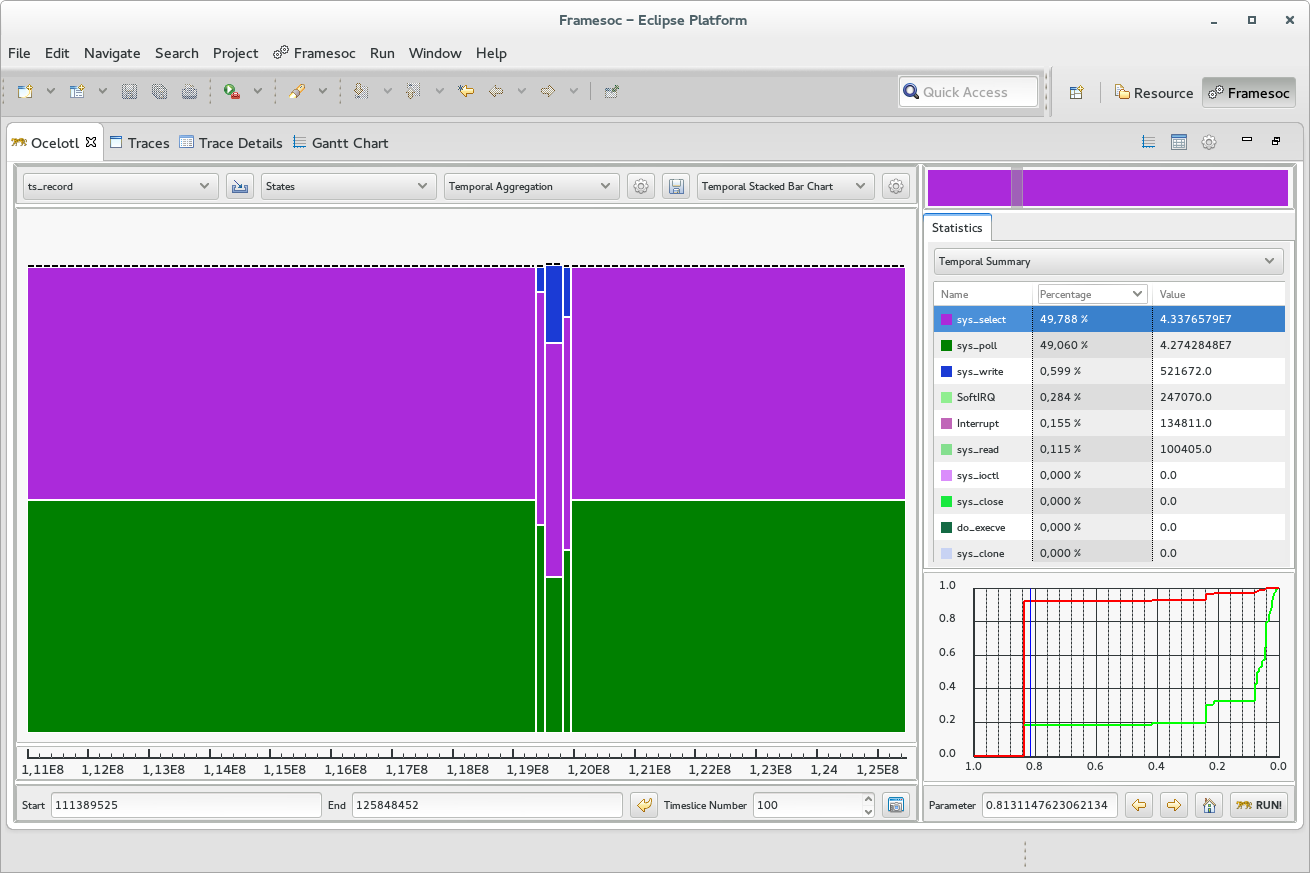
\includegraphics[width=\textwidth]{img/ocelotlt}
\end{minipage}
\vfill
\begin{minipage}[c]{0.80\textwidth}
  Example of a temporal overview provided by Ocelotl, a tool I 
designed during my Ph.D. This visualization is built upon an aggregation 
technique based on information theory measures. It gives feedback about the 
homogeneous temporal parts of an application execution trace, and helps to find 
phases, perturbations and problematic behaviors, even for huge traces that can 
not be represented with classic visualization techniques. The tool can be 
downloaded at
\href{http://soctrace-inria.github.io/ocelotl/}{
http://soctrace-inria.github.io/ocelotl/}
\end{minipage}
\vfill
\begin{minipage}[c]{0.70\textwidth}
 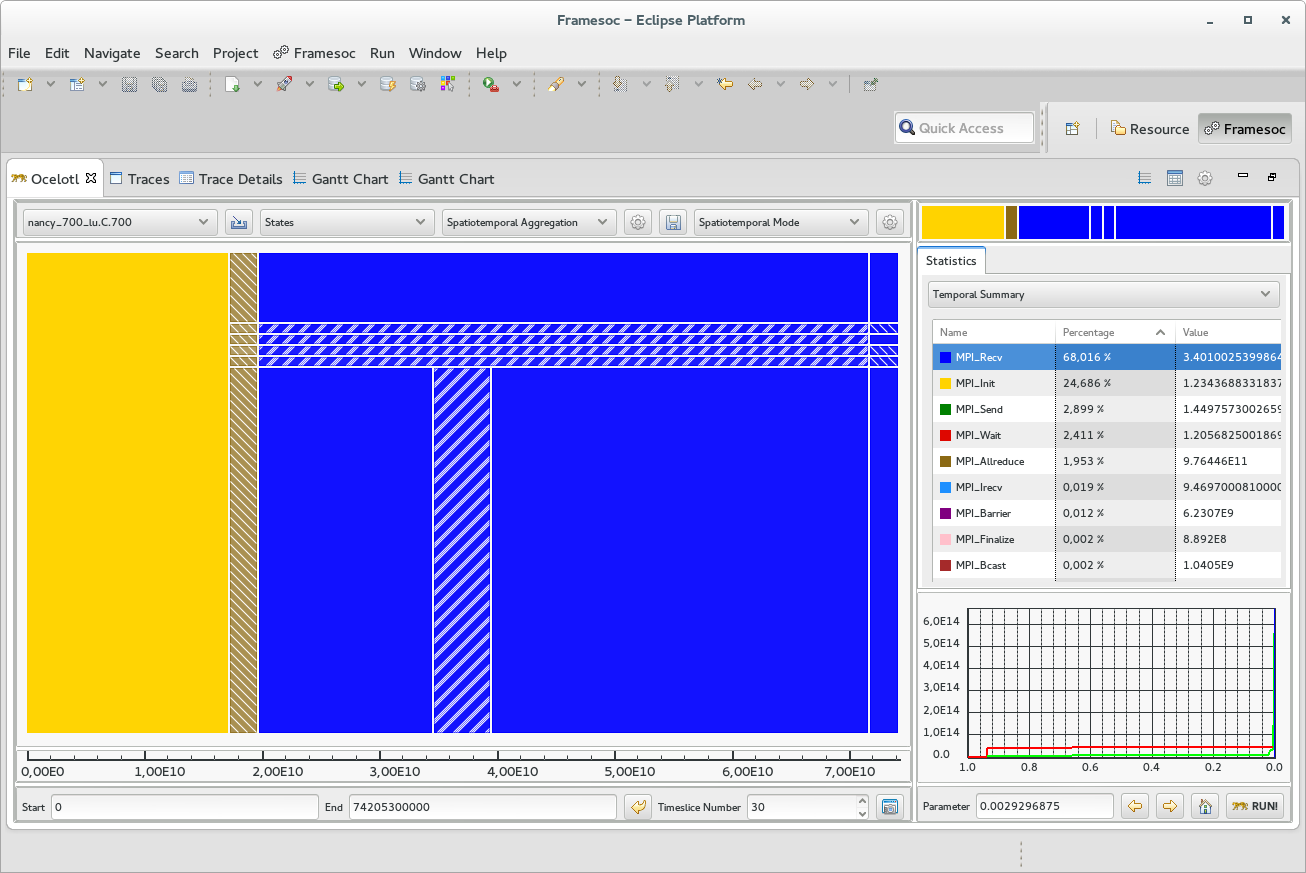
\includegraphics[width=\textwidth]{img/ocelotlst}
\end{minipage}
\vfill
\begin{minipage}[c]{0.80\textwidth}
We also propose a spatiotemporal overview based on 
the same principle. Our objective is to correlate the application 
behavior with the different hardware and software components involved in its 
execution. The trace showed here is a 15 GB file containing 218 million 
events, get from the execution of a 700 process MPI application.
\end{minipage}
\vfill
\raggedright

